\documentclass{article}
\usepackage{graphicx}
\usepackage{threeparttable}
\usepackage{amssymb}
%% xcolor has nicer colours than default
\usepackage[dvipsnames]{xcolor}
\usepackage[backref,breaklinks,colorlinks,citecolor=Blue,linkcolor=Blue,urlcolor=Blue]{hyperref}
\usepackage{pdflscape}

\title{Concepts of function in biology and biomedicine}
\begin{document}
\maketitle

\section{Abstract}
\label{sec:abstract}

Several philosophical accounts of disease are constructed at least partly around the idea that disease is a failure of physiological parts or processes to perform their biological function or an ``impairment of normal functioning''. Determining whether a phenotype—such as obesity—is a disease or determining the level of functioning at which some aspect of physiology—such as response to insulin—becomes pathological throws considerable weight on the concept of biological function. However, there are a number of philosophical theories of biological function, each of which defines function differently. It is not clear which theory—or combination of theories—we should use to explicate the medical conception of function. One reason for this is that we have no systematic way to determine how biologists and medical practitioners conceive of, or write about, function in their respective disciplines. To further complicate matters, natural language is replete with ambiguities, and scientific manuscripts often use technical terms imprecisely. Without a descriptive understanding of how different conceptions of function are used in biology and medicine, we have little hope of bringing insights about biological function to bear on disputes about function and malfunction in medicine. Here we develop a systematic method for analysing references to function by outlining a classification scheme that combines syntactic and semantic analysis in a dependency-grammar framework.

\section{Introduction}
\label{sec:introduction}

Much of philosophy of medicine is concerned with issues surrounding the concept of disease.
Philosophical approaches to categorising disease can be broadly divided into two camps: a normativist view that prioritises social value judgements and a naturalist view that prioritises biological theory.\footnote{There are also hybrid views, such as Wakefield's harmful dysfunction account \cite{wakefield1992}. }
The former contends that judgements about disease should be primarily based on whether society disvalues the condition in question, whereas the latter holds that our categorisation of disease should be primarily based on whether ``something has gone wrong'' in a biological system \cite{matthewson2017} .
But what does it mean for ``something to go wrong'' with a biological system according to the naturalist view?

Before determining what it means for ``something to go wrong'', one requires a normative framework that can be used to determine what a biological component (trait) ought to do  .
To ground normative claims in biology, many naturalist accounts defer to the notion of function.
If a trait's function is what the trait ought to do, then a dysfunctional trait no longer does what the trait ought to do.
But herein lies several problems.
Function is a word with multiple senses in both its colloquial and discipline-specific uses.
Within the discipline of philosophy, there are many theories of biological function, each differing in their claims to normativity (and some with arguably no normative claims whatsoever).
In more applied disciplines, such as biology, medical research, and clinical medicine, it can be unclear which concept of function is being employed or how well usage maps onto philosophical conceptions of function.

Experimental philosophy relies, in large part, on extracting meaning from natural language.
If we hope to use experimental philosophy to understand a naturalistic account of disease and dysfunction, we must first clarify how the concept of function (and dysfunction) is used in natural language.
%It is thus crucial that philosophers have methods for identifying which sense of function is used in natural language.
One must solve two broad problems in order to consistently disambiguate real-world usage of biological function (or any word that refers to multiple concepts).
First, one must develop a classification scheme comprising a set of categories, each of which defines a sense (or concept) of function.
The categories within the set should be exhaustive, covering all possible real-world uses of function.
Furthermore, the categories should either be exclusive (i.e. each use of function has one and only one sense) or there should be explicit rules for how one is to deal with membership in overlapping categories (e.g. a hierarchy of definitions or allowing of multiple senses for a single usage). 
Second, one must develop a system that can consistently assign a piece of natural language on biological function (sentence, paragraph, etc.) into its correct category.

The problem of developing a set of categories will typically employ some form of conceptual analysis (and/or leverage earlier conceptual analysis).
We cannot, however, simply paste together existing concepts of biological function.
For one, this will not necessarily generate a set of function concepts that are exhaustive or exclusive.\footnote{For an example with respect to exclusivity, consider that some philosophical concepts of function have closely overlapping features. Say we have two overlapping concepts, such as the causal role and organisational theories of function. We must make some hard decisions when deciding how to incorporate these concepts into a coherent classification scheme. We could choose one category and remove the other, allow both but give one hierarchical precedence over the other when ambiguities arise, allow a single usage to be assigned to both categories, or create a general category that encompasses both concepts. (Here we have chosen the latter approach.)}
Moreover, real-world usage of function does not always align with philosophical concepts of function.
A classification scheme for experimental philosophy will thus necessarily be an amalgamation of philosophical conceptual analysis and discipline-specific usage.

A study has recently attempted this for biological function in the context of de novo gene emergence (cite elife).
The authors chose six categories for their classification scheme: Evolutionary Implications, Physiological Implications, Interactions, Capacities, Expression, and Vague.
The authors started broadly with the two most well-known philosophical concepts of function: causal role and selected effects.
From this base, they iterated through a small dataset of 42 examples (from 20 abstracts), adding categories and refining the scheme as they encountered new usages that did not fit into the existing scheme.
They achieve an exhaustive scheme by implementing a catch-all category of Vague for usage unable to be categorised in one of the other five categories.
They did not require that these categories be mutually exclusive, instead allowing a single usage to have membership in multiple categories.
To categorise each usage of function using the scheme, the authors started by independently reading a paper's title and abstract.
Next they used a list of definitions to assign at least one meaning of function to the example, which were supplemented by a few general coding rules to guide application of the definitions.
One of the most striking findings from this study was the difficulty of obtaining agreement between the different raters: in only 12\% of cases did all four raters independently assign an example to the same category!\footnote{In addition, the authors used 17 of the 20 abstracts to develop their classification scheme, meaning that their reported level of agreement---which was based on all 20 abstracts---is almost certainly higher than they would achieve on a never-before-seen set of abstracts on de novo gene function (in the parlance of statistics and machine learning, their reported result is ``overfit'' on account of them using the same data for training and testing).}
After conferring with one another and employing a consensus-based approach, the raters were still only able to assign 62\% of cases to a single category.
Despite having a comprehensive and well-reasoned classification scheme in hand, these authors were not able to consistently categorise real-world usages of function into a single category.
This is clearly an immensely difficult problem to solve, and there are likely a number of factors that contributed to the difficulty in unambiguously assigning usages of function to a single concept.
We suggest, however, that a crucial factor lies in the different ways that individual investigators analyse natural language in order to extract meaning.
Without a detailed and standardised framework, the semantic mapping from natural language to a definition of function is bound to be inconsistent among different investigators.

In this manuscript, we ask a similar question to Keeling et. al. (2019) but adopt a different methodology.
Our classification scheme does not try to semantically map directly from natural language to definitions of function.
To assign an example to a definition, one instead follows a step-by-step flowchart, answering questions and identifying important features related to function that are contained within a piece of natural language.
We unpack each piece of natural language into one of several common forms.
For example, to be classified as Biological Role (see section ``Senses of function''), an investigator must be able to identify each variable in the unpacked form of ``The function of \emph{ITEM} is \emph{EFFECT} in \emph{SYSTEM}'' (e.g. \emph{ITEM} could be ``The heart'', \emph{EFFECT} could be ``to pump blood through'', and \emph{SYSTEM} could be ``the circulatory system'').
By simplifying natural language into simple, common forms, our approach avoids obfuscation of meaning due to variation in syntactic construction and helps standardise the technique for extracting meaning.
Moreover, we provide detailed instructions for how to use the dependency grammar framework and modern natural language processing techniques as aids in identifying the variables in the common forms.

\section{Classification scheme}
\label{sec:class-scheme}

Our approach was to analyse real-world uses of biological function extracted from scientific papers.
Since our focus was on how function is used in biology, we used examples from a wide variety of biological subfields.
We used the Australian Research Council Field of Research codes to identify the following biological subfields: biochemistry and cell biology, ecology, evolutionary biology, genetics, microbiology, physiology, plant biology, and zoology.
We matched these subfields to the following fields from Clarivate Analytic’s Web of Science database: biochemistry and molecular biology, ecology, evolutionary biology, genetics and heredity, microbiology, physiology, plant sciences, and zoology.
In addition, we considered the general biology category and the general science category.
We used Clarivate Analytic’s Journal Impact Factor (JIF) to get a ranking of journals, and for each category, we chose the top five journals by JIF (\href{https://github.com/joshuachristie/function-concepts/blob/master/supplementary_material/list_of_journals.txt}{\underline{supplementary material: journal list}}).
We searched within Web of Science using the search string ``function*'' for journals from the biological subfield categories and ``biolog* AND function*'' for journals from the general biology and general science categories.
We chose the first listed paper from each journal, and we extracted all sentences involving a use of function from the full texts (ignoring abstracts), giving us 1316 usages of function that we used to develop our scheme.

Developing a classification scheme is a difficult proposition, as the process unavoidably involves circularity: in order to create a scheme that can classify examples, we first need a set of classified examples that we can use to test and iteratively develop the scheme.
How can we confidently classify examples before we have a scheme to classify examples?
We used two main methods to obtain a set of ``gold-standard'' examples that we could use to help develop our scheme.
In the first method, three of the authors (JRC, ZW, SG) independently analysed a subset of the sentences using definitions and a simple set of classification guidelines (much like the approach taken in Keeling et. al. (2019)).
We then compared our responses, and if our classifications differed, we used a consensus-based approach to categorise examples.
Those examples that all of us were confident about formed a set of gold-standard examples.
A disadvantage of using a consensus-based approach is that we can never be sure of the author's intentions, even in examples that we confidently and unanimously categorised.

The second method we used was to simplify real sentences that we encountered, using these examples as a base from which to write (and rewrite) our own sentences.
Say we have a sentence that we decide (through consensus) is used in the sense of Biological Role.
We can simplify the sentence and rewrite it using different syntactic structures (but retaining the sense of Biological Role).
Moreover, we can change the sentence such that it now instead expresses Biological Advantage (and again rewrite it multiple times using different syntactic structures).
This approach has two main benefits over the consensus-based approach: (i) with these examples we know with certainty the author's intentions, having purposefully written them ourselves to fit a specific category; and (ii) by exploring different syntactic structures, we help ensure that our classification scheme is robust to alternate phrasings.
In addition to obtaining these gold-standard examples, we also set aside interesting cases that were problematic to classify.
We iteratively modified our classification scheme so as to handle these problematic cases and other generally problematic patterns that arose repeatedly (altering the flowchart, adding new categories, modifying the natural language analysis, and so on).

\subsection{Senses of function}
\label{sec:senses-function}

The first step was to choose the categories of our classification scheme.
We decided to use the scheme of Wouters (2003) as our starting point.
Wouters breaks down function into four categories: (i) Biological Activity; (ii) Biological Role; (iii) Biological Advantage; and (iv) Selected Effect.
In Wouters's scheme, Biological Activity is ``what an item does or is capable of doing'', Biological Role describes ``how a certain item or activity contributes to the emergence of a complex capacity of an organism'', Biological Advantage refers to the ``biological value (utility) of a certain trait in comparison with another'', and Selected Effect is ``used in a historical sense to refer to the effects for which a certain trait was selected in the past''.

We added a new category of function whenever we encountered instances of usage that reoccurred multiple times and could not be classified in one of our existing categories.
To Biological Activity, Biological Role, Biological Advantage, and Selected Effect, we added the following categories: Colloquial, Technical, and To Work.
In some instances, the sentence does not contain sufficient information to identify all the variables.
We thus added the following additional categories whose purpose is to specify which feature is missing from the sentence: Description Incomplete: \emph{ITEM} Unspecified, Description Incomplete: \emph{EFFECT} Unspecified, and Description Incomplete: \emph{EFFECT} Specified.
The classification scheme flowchart is shown in Figure \ref{flowchart} and descriptions of the decision points are in Table \ref{tab:flowchart}.

\begin{figure}[ht]
  \centering
  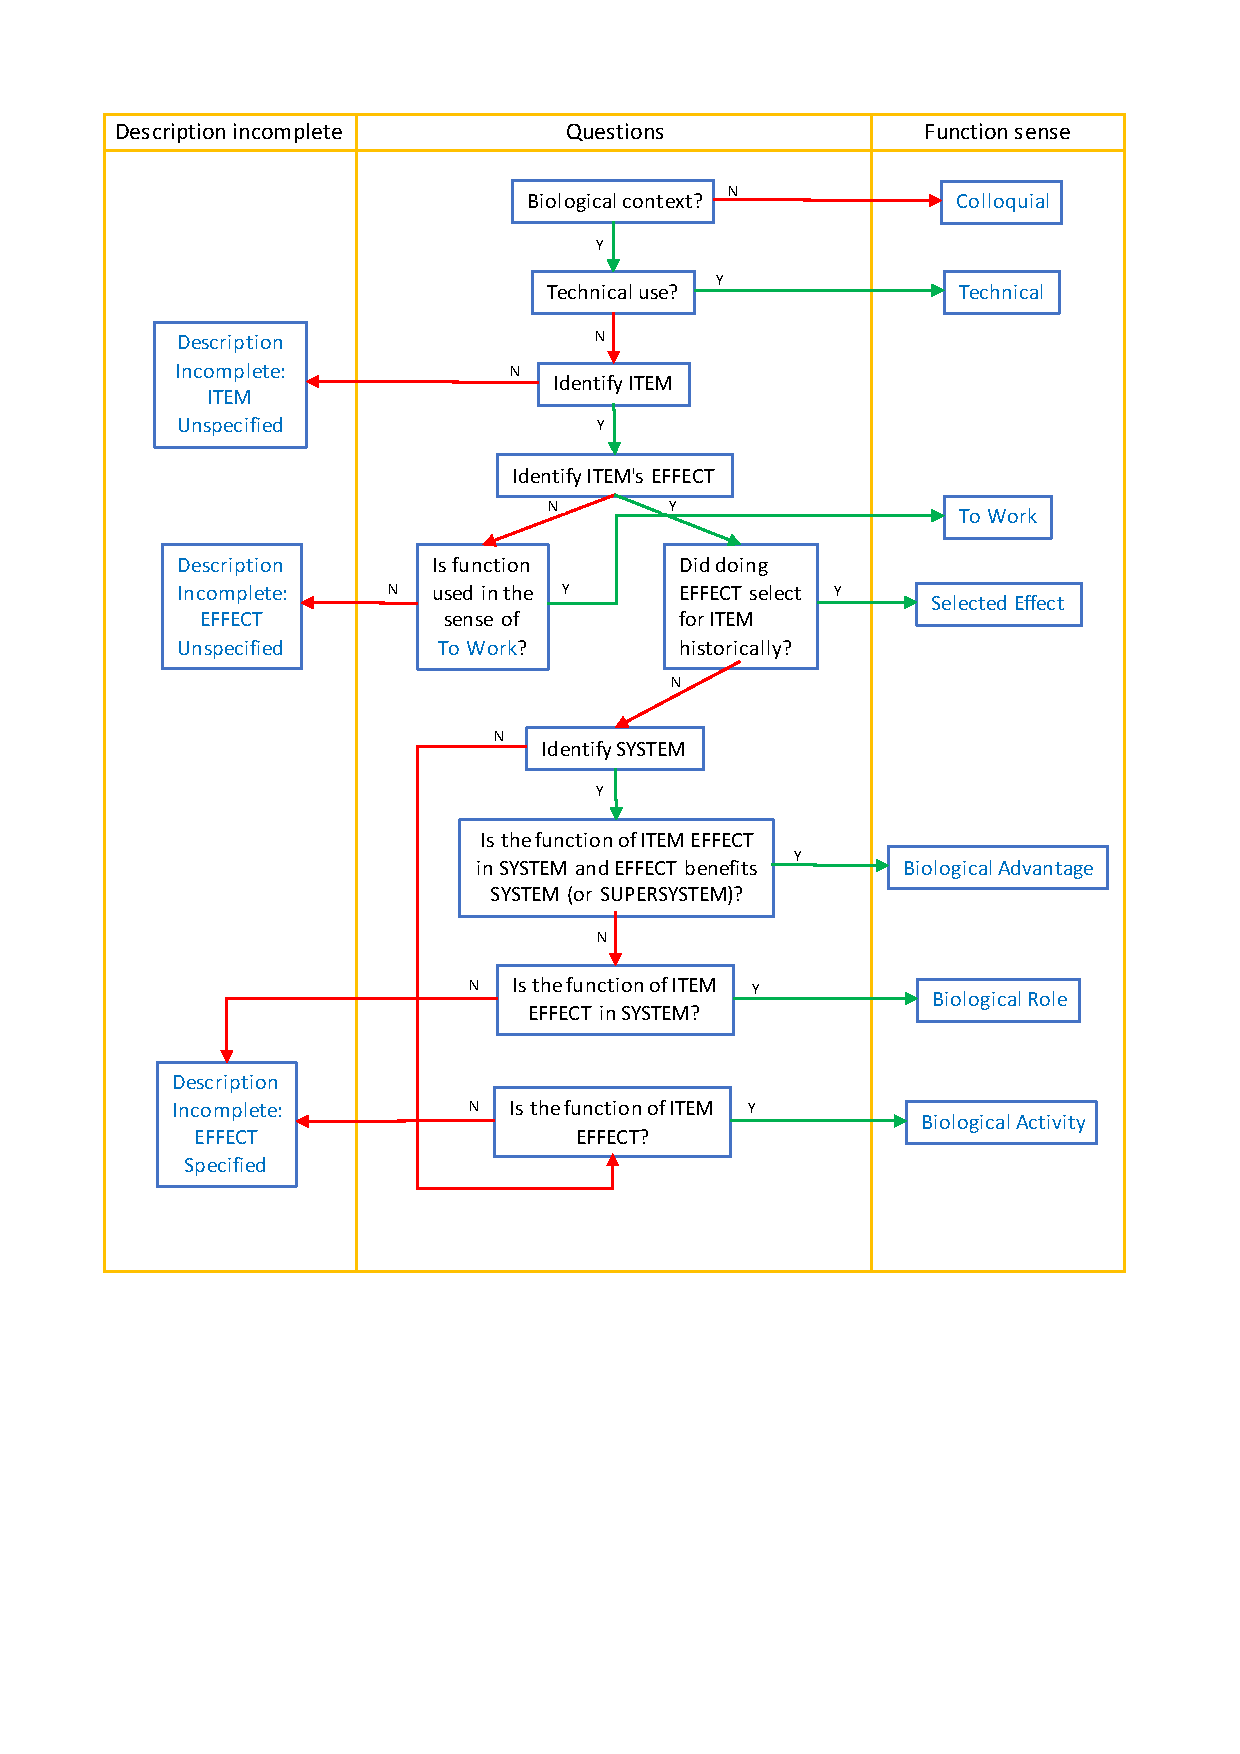
\includegraphics[width=\linewidth]{figures/GeneralFlowchart.pdf}
  \caption[\textbf{Decision flowchart for identifying sense of function.}]{}
  \label{flowchart}
\end{figure}


\begin{landscape}
  \begin{table}
    \small
    \caption{Description of each decision point in the classification flowchart (Figure \ref{flowchart})}
  \begin{tabular}{|p{0.17\linewidth}|p{0.97\linewidth}|}
    \hline
    Decision point & Description \\
    \hline
    Biological context? & Are we dealing with a case of biological function or colloquial use (see \href{http://wordnetweb.princeton.edu/perl/webwn?s=function&sub=Search+WordNet&o2=&o0=1&o8=1&o1=1&o7=&o5=&o9=&o6=&o3=&o4=&h=}{WordNet 3.1} for colloquial definitions)? These examples are rare if one restricts the corpus to scientific papers in biology. Notable exceptions are mathematical functions and programming functions, which we place within Colloquial to simplify the flowchart. \\
    \hline
    Technical use? & Compound phrases such as ``functional ecology'', ``functional biology'', ``functional connectivity'', and so on. These phrases will be familiar to practitioners within a field. Their meanings are multi-faceted and influenced by a field's development and cannot be meaningfully unpacked using a flowchart.  These phrases will often appear multiple times in a manuscript. \\
    \hline
    Identify \emph{ITEM} &  An \emph{ITEM} is something that can be a character or trait (or produced by one) of a Darwinian individual. Obvious candidates are concrete nouns, which refer to a physical item (e.g. heart), but it also includes abstract nouns if they refer to a concrete concept (e.g. ``gene'' as used in population genetics, ``boldness'' as a behavioural phenotype, etc.). Importantly, there must be a dependency between function and the \emph{ITEM}---it is not sufficient that a suitable \emph{ITEM} simply appear in the sentence (e.g. ``protein'' is the \emph{ITEM} in  ``protein function aids muscle development'' but ``muscle'' is the \emph{ITEM} in ``protein aids in muscle function''). \\
    \hline
    Identify \emph{ITEM}'s \emph{EFFECT} & \emph{EFFECT} is what the \emph{ITEM} does (or, less commonly, has done to it). \emph{EFFECT} is a verb or verb phrase, or it is a word or phrase that can be converted into a verb (e.g. ``contribute to transcription'' could be converted to the verb ``transcribe''). \emph{EFFECT} must be a concrete action or effect of the \emph{ITEM} (e.g. if \emph{ITEM} is ``gene'' then ``is transcribed'' is acceptable but ``benefits health'' is not). \\
    \hline
    Is function used in the sense of To Work? & A heuristic is whether you can substitute ``\emph{ITEM} function'' (or equivalent, depending on the sentence) with ``how well \emph{ITEM} performs'', ``a working \emph{ITEM}'', or similar into the raw sentence without loss of meaning. For example, ``Liver function is important for health'' might become ``A working liver is important for health'' without loss of meaning.\\
    \hline
    Did doing \emph{EFFECT} select for \emph{ITEM} historically? & Can it fit the following form: the function of \emph{ITEM} is to \emph{EFFECT} such that doing \emph{EFFECT} in the past caused \emph{ITEM} to be selected or maintained in a population (relative to an actual or counterfactual historical alternative to \emph{ITEM})? An example would be ``zebra stripes are functional because they evolved to reduce insect bites'' as reducing insect bites (\emph{EFFECT}) has selected for zebra stripes (\emph{ITEM}).\\
    \hline
    Identify \emph{SYSTEM} & A \emph{SYSTEM} is either a Darwinian individual, or a complex system within an individual, that contains the \emph{ITEM}. The \emph{EFFECT} of the \emph{ITEM} on the \emph{SYSTEM} contributes to a capacity of the \emph{SYSTEM}. As a heuristic for identifying the \emph{SYSTEM}, you can ask  ``how does \emph{ITEM} produce \emph{EFFECT}?'' or ``for what is \emph{ITEM} producing \emph{EFFECT} used?''. \\
    \hline
    Is the function of \emph{ITEM} \emph{EFFECT} in \emph{SYSTEM} and \emph{EFFECT} benefits \emph{SYSTEM} (or \emph{SUPERSYSTEM})? & Consider ``Transcript X functions to regulate expression in the liver, which improves liver performance through regulation of glycogen storage.''. We can unpack this as ``The function of \emph{TRANSCRIPT X} is to \emph{REGULATE EXPRESSION} in \emph{GLYCOGEN STORAGE IN THE LIVER} and \emph{REGULATING EXPRESSION} benefits [improves performance of] \emph{THE LIVER}''. Note the statement's contrastive nature: ``improves liver performance'' indicates that transcript X is being compared to an (unstated) alternative (e.g. transcript Y). Although contrast will often occur, it is not required. For example, we would still classify this example as Biological Advantage if we replaced ``improves liver performance'' with ``aids metabolic control''. Although this alteration removes the contrast, it nevertheless describes a benefit to a supersystem (metabolic system). (A \emph{SUPERSYSTEM} is a system that contains \emph{SYSTEM} up to and including the level of a Darwinian individual.) \\
    \hline
    Is the function of \emph{ITEM} \emph{EFFECT} in \emph{SYSTEM}? &  Biological Role is not contrastive, and it does not contain language indicating a benefit to a system (or supersystem). An example is ``Transcript X functions to regulate expression in the liver, which plays a role in regulation of glycogen storage''. This statement neither contrasts transcript X with an alternative---it simply describes how transcript X contributes to a capacity of the \emph{SYSTEM}---nor explicitly describes a benefit to the \emph{SYSTEM}.  \\
    \hline
    Is the function of \emph{ITEM} \emph{EFFECT}? &  Biological Activity is Biological Role without a \emph{SYSTEM} being specified. An example is ``Transcript X functions to regulate expression'', which simply describes what transcript X does. We do not know how (or in what system) it is being used. \\
    \hline
  \end{tabular}
  \label{tab:flowchart}
\end{table}
\end{landscape}

\subsection{Biological Activity, Role, and Advantage}
\label{sec:relat-betw-funct}

The categories of Biological Activity, Biological Role, and Biological Advantage are conceptually related.
The relationship between Biological Activity and Role is straightforward: a Biological Role is a Biological Activity that contributes to the capacity of an organism (or, more generally, to the capacity of a system). 
The difference between Biological Role and Biological Advantage is summed up, in Wouters's words, by ``a distinction between 'how it is used' (role) and 'how it is useful' (advantage)'' (wouters2003).
We can thus think of Biological Advantage as a Biological Role that benefits an organism by virtue of contributing to a capacity of a system (of that organism).

We classify these three categories in a hierarchical manner, such that Advantage $>$ Role $>$ Activity.
By this we mean that if an example is classified as Biological Advantage, it has also satisfied the criteria for Role and Activity, and if classified as Role, then it has also satisfied the criteria for Activity.
There are three benefits behind our approach: (i) it neatly captures the relation between these categories within the context of our classification process, as each category is associated with identifying additional feature(s) (\emph{ITEM} and \emph{EFFECT} for the base category of Biological Activity, \emph{SYSTEM} for Biological Role, and a benefit of \emph{EFFECT} toward \emph{SYSTEM} (or \emph{SUPERSYSTEM}) for Biological Advantage); (ii) it is an effective method for developing a classification with mutually-exclusive categories (there would be significant overlap without a hierarchical system, e.g. every Biological Role would also be a Biological Activity); and (iii) it allows for categories to be easily combined \emph{post hoc} if desired (see next section for an example).

\subsubsection{Biological Activity}
\label{sec:biological-activity-1}

Biological Activity answers the question ``what does it do?''.
It was first(?) described by Neander (1995) as ``minimal function''.
It deals with biological characters (e.g. a biological item, feature, or behaviour), describing what these characters do (or are capable of doing) (Wouters2003).
It has received relatively little philosophical attention, likely because a statement of Biological Activity leaves out important information about how the character is used or why it exists.
Indeed, Biological Activity is often ignored or subsumed under Biological Role, with the resulting category typically being termed ``causal role'' function \cite{cummins1975} .
We have chosen to keep this distinction for two main reasons.
We believe that Biological Activity does reflect some actual biological use, notably in the ENCODE study whose goal was to map functionality across the human genome (encode2012).\footnote{It is commonly stated that ENCODE used a causal role definition (e.g. cite1, cite2), but we believe this to be a conflation of Biological Activity and Biological Role. ENCODE focused on correlates of biological activity (encoding protein or non-coding RNA, or displaying a biological signature such as protein binding or a specific chromatin structure) without trying to establish how this activity is used to generate a complex capacity in the wider system.}
Second, keeping the distinction preserves information.
If an investigator believes that the distinction between Biological Activity and Role is spurious, then they can always combine (labelled examples of) the two categories into a single category during the analysis phase.
But one cannot separate these categories \emph{post hoc} if they were originally classified as a single category.

\subsubsection{Biological Role}
\label{sec:biological-role}

Biological Role answers the question ``how is it used?''.
It is closely linked to causal role or mechanistic theories of function (e.g. Cummins 1975, Wouters also cites Bechtel/ Richardson 1993 and Craver 2001).
Like Activity, it deals with biological characters (wouters2003), describing how a character's effect can contribute to a capacity of a complex system.
In addition to causal theories, some real-world uses of organisational theories of function (mossio2009) will likely fall under Biological Role.
Organisational theories differ from causal theories in that they use the notion of a closed and differentiated self-maintaining organisation as a basis for teleology and normativity.
But organisational theories might be classified as Biological Role if the self-maintenance aspect is omitted or downplayed in a particular usage.

\subsubsection{Biological Advantage}
\label{sec:biological-advantage}

Biological Advantage answers the question ``how does it help?''.
It is closely linked with [see garson2016, who calls it fitness-contribution, for some different theories under this broad umbrella; mossoi2009 also mentions Bigelow and Pargetter [1987]; Canfield [1964]; Ruse [1971]].
In Wouters's characterisation, Biological Advantage deals with traits (specific variants of a character), and it is contrastive in nature, describing how a trait's effect has benefits relative to an alternative trait.
Wouters's interpretation of advantage is somewhat more general than the aforementioned theories that focus explicitly on fitness benefits for Darwinian individuals.
Wouters's definition requires that an \emph{ITEM} demonstrate biological value (or utility) over an alternative.
While Wouters states that the ultimate benchmark for biological value is fitness, he acknowledges that Biological Advantage statements may simply describe ``the efficiency with which a certain biological role is performed''.
In these sorts of statements, there is an implicit assumption that improved efficiency of this role benefits the individual, and that it does so in such a way that it correlates with fitness.
This approach will thus include false-positives in cases where the benefits identified correlate poorly with fitness.
In practice, this means that Wouters's characterisation of Biological Advantage is quite permissive, being satisfied if an organism can do \emph{EFFECT} better with \emph{ITEM} than with an alternative trait.

Some have argued, in opposition to Wouters, that Biological Advantage need not be contrastive (or be limited to dealing with traits), instead focusing on how it contributes to survival (garson2016 referencing buller1998).
There are obvious parallels between a non-contrastive view of Biological Advantage and organisational theories of function, which focus on how an \emph{ITEM}'s \emph{EFFECT} contributes to self-maintenance [a non-contrastive benefit] of a \emph{SYSTEM}.
With this in mind, we take a very general view of Biological Advantage, adopting Wouters's permissive interpretation of biological advantage as improving a biological role's efficiency without requiring that the characterisation be contrastive.\footnote{We also found that a strict philosophical interpretation of Biological Advantage meant that it could be difficult to identify all the requisite components within a sentence, leading to few examples being characterised as Biological Advantage.}
For our purposes, any explicit mention of a benefit to a system of a Darwinian individual is sufficient for an example to be categorised as Biological Advantage instead of Biological Role.
Usages of organisational theories explicitly mentioning the benefits of self-maintenance will thus fall under Biological Advantage (as mentioned previously, those usages of organisational theories that omit explicit references to the benefits of self-maintenance will likely fall under Biological Role).

\subsection{Function as To Work}
\label{sec:funct-as-perf}

We identify another common use of function, namely that of To Work.
In our flowchart, this use of function can only arise when the \emph{EFFECT} of an \emph{ITEM} is not specified (Figure \ref{flowchart}).
This use has an analog in one of the colloquial senses of function, namely ``to work as expected''.
Function as To Work is primarily concerned with how an item has developed in individuals, and whether it is deemed to be functional (in the sense of working as expected) or dysfunctional (not working as expected).
This use of function differs from Biological Activity, Role, Advantage, and Selected Effect, which are all ``type'' level designations (dealing with lineages of characters or traits).
Function as To Work instead focuses on token level ascriptions (traits of individuals), and it is concerned with the development and manifestation of traits or systems in individuals.\footnote{Of course, dysfunctions are also applied to groups of individuals by virtue of being categorised into diseases or syndromes.
But to the degree that diseases or syndromes cluster traits and systems, they primarily do so based on similarities in how or why ``things have gone wrong'' rather than on lineages of characters or traits.
(There are, admittedly, some difficult cases, such as genetic disorders like mitochondrial disease, in which a disease will cluster traits in a manner more akin to Selected Effect lineages. In these cases, the line between novel type traits and dysfunctional token traits becomes blurred.)}

An example of this usage is ``liver function is important for an individual's health''.
Here function does not refer to a function of the liver (e.g. ``the liver functions to store glycogen''), but to the \emph{functioning} of the liver.
We could, for example, express the same meaning in the revised phrase ``a liver that works as expected is important for an individual's health''.
An item that ``works as expected'' is one that aligns with the naturalist view of ``healthy'' or ``absence of disease''.
It implies that there exists a normative basis for believing how the item ought to function.
The normative basis might derive from a philosophical theory, such as selected effects or the organisational theory, but it might have another basis entirely.
Consider a statement such as ``The gene is transcribed and thus is functional''.
What is the normative basis behind this statement?
It appears to adopt some form of a Biological Activity definition, namely that for function it is sufficient that a gene (item) is transcribed (effect) without regard for how it is used within a system.
There might be an explicit set of criteria behind this definition---as in the ENCODE project---but frequently the appeal to normativity will be implicit (and its justification may be less than sound).
In the statement above, the author may simply have a vague sense that any gene that does something is functional, perhaps as a complement to the notion that a non-functional gene is one that does nothing.
Few scientific papers that use ``function'' explicitly define it, making it difficult to infer a normative basis in short pieces of natural language.
For the To Work category, we focus on whether a normative basis is expressed by the author's language.
The function use itself may indicate the normative basis, as with ``dysfunction'', ``malfunction'', ``loss of function'', and so on.
But oftentimes the appeal to normativity will be more subtle.
For practical reasons, we choose to be agnostic as to how the normative basis is constructed.

\section{Analysis of natural language}
\label{sec:analys-natur-lang}

Function has many derivatives (e.g. functional) and can be used in different parts of speech (noun, verb, etc.), which significantly complicates analysis of natural language.
If we focus just on the forms of function when used as a noun, we have the singular ``function'' (``the function of the heart''), and the plural ``functions'' (``the heart has many functions''), and the derivative ``functionality'' (``the functionality of the heart'').
Grammatical relations also vary.
In ``the function of the heart'' and ``the functionality of the heart'', function is the subject, whereas for ``the heart has many functions'', function is the direct object.
Aside from its use as a noun, ``functions'' (and ``function'') can also be used as a verb (``the heart functions to pump blood'').
We also encounter cases such as the gerund form ``functioning'', which is the -ing form of the verb ``function'' that acts as a noun (``functioning is important for hearts'')!
And to complicate matters even further, ``functioning'' might be a present participle instead of a gerund, in which case it either acts as an adjective (``the functioning heart'') or to form verb tense (``the heart was functioning''). Suffice it to say, when dealing with real-world sentences, the sheer variety of syntactical forms present a challenge for semantic interpretation of function.
A central component of our approach is to simplify these diverse syntactic constructions into the common forms highlighted in Figure \ref{flowchart} and Table \ref{tab:flowchart}.
 
To simplify comparison of syntactically-diverse constructions, we use word conversion to convert from derivations of function (e.g. functional) to its morpheme form ``function''.
We will use morphological derivation to convert between parts of speech (e.g. adjective to noun) and inflection to convert between number, tense, and aspect (e.g. the plural ``functions'' to ``function'').
During conversion, it is crucial that we retain the syntactic dependencies between the function use and other parts of speech, as these form the basis for identifying the variables in the unpacked form (\emph{ITEM}, \emph{EFFECT}, etc.).
We use a grammatical framework called dependency grammar (cite that recent review), which structures grammatical relations as directed links between words.
Effectively, these syntactic dependencies constrain the parts of a sentence that can be chosen as \emph{ITEM}, \emph{EFFECT}, and so on.
To see why this is necessary, consider a statement such as ``Protein function aids muscle development''.
There is a syntactic dependency between ``protein'' and ``function'' (``protein function'' is a compound noun).
If we were to ignore syntactic dependencies, then ``protein'' and ``muscle'' would be equally good candidates for the \emph{ITEM}, as both are biological items.
In this case, ``protein'' is the correct \emph{ITEM} due to its dependency with ``function''.
If we had chosen ``muscle'' instead, we would have unintentionally altered the meaning of the sentence, rendering our analysis of function incorrect.
(In this example, it is trivial to use intuition to see that ``protein'' should be the \emph{ITEM}, but in real natural language it is frequently difficult to establish this connection through intuition alone.)
Our goal is to use syntactic dependencies (starting from function or its derivative) to unpack a sentence such that the correct semantic relations can be cast into a standard form.

\section{Analysis of function sentences}
\label{sec:example-sentences}

In this section, we work through six examples using our classification scheme and natural language analysis.
We use the natural language processing software \texttt{spaCy} to label parts of speech (noun, verb, and so on) and to generate the dependency grammar representation \cite{spacy}.
We focus on short toy sentences to illustrate the framework, giving a general overview of the natural language analysis without providing the explicit rules.
To download the software, explore some more detailed examples, or to read a handbook detailing the rules governing the natural language analysis, see
\newline
\href{https://github.com/joshuachristie/function-concepts}{https://github.com/joshuachristie/function-concepts}.

\begin{figure}[ht]
  \centering
  
\includegraphics[width=\linewidth]{figures/combined_eff_role_adv.png}
  \caption[]{\textbf{Dependency grammar analysis of Biological Activity (A), Role (B), and Advantage (C).}}
  \label{eff_role_adv}
\end{figure}

\subsection{Biological Activity}
\label{sec:biological-activity}

Let us work through the flowchart (Figure \ref{flowchart}) using the sentence ``The transcript functions to regulate expression'' (Figure \ref{eff_role_adv}A).
Here ``functions'' is used as a verb.
There is a dependency---represented by an arrow---between functions and ``transcript'' (of type \texttt{nsubj}, nominal subject).
Given this dependency, and the fact that ``transcript'' is a product of a trait of a Darwinian individual, we can identify ``transcript'' as the \emph{ITEM}.
There is also a dependency (via \texttt{xcomp}, a clausal complement) between the verb ``functions'' and the transitive verb ``to regulate'' which takes ``expression'' as its direct object.
Since ``to regulate expression'' is what the \emph{ITEM} does (and it is a concrete action or effect), we can identify it as the \emph{EFFECT}.
There is no language indicating historical selection, and we cannot identify a \emph{SYSTEM}.
Since we have identified the \emph{ITEM} and \emph{EFFECT}, by following Figure \ref{flowchart} we get the unpacked form ``The function of the \emph{TRANSCRIPT} [item] is \emph{TO REGULATE EXPRESSION} [effect]'', which gives a classification of Biological Activity.

\subsection{Biological Role}
\label{sec:biological-role-1}

Consider the sentence ``The transcript functions to regulate expression in metabolism.'' (Figure \ref{eff_role_adv}B), which differs from the previous one by the addition of the prepositional phrase ``in metabolism'' (marked by \texttt{case}).
As before, the \emph{ITEM} is ``transcript'' and the \emph{EFFECT} is ``to regulate expression'', and there is no language indicating historical selection.
Unlike before, there is now a dependency between ``expression'' (part of the \emph{EFFECT}) and the noun of the prepositional phrase ``metabolism'' (via \texttt{nmod}, nominal modifier).
(This dependency provides information about the \emph{EFFECT} and answers the question ``how is it used?'' with ``in the metabolic system''.)
Since ``metabolism'' represents a complex system (metabolic system) in which the transcript plays a role, we can identify \emph{SYSTEM} as ``metabolic system''.
There is no language that indicates a benefit to the metabolic system (or a supersystem containing it), and so we unpack it as ``The function of the \emph{TRANSCRIPT} [item] is \emph{TO REGULATE EXPRESSION} [effect] in the \emph{METABOLIC SYSTEM} [system]'', which gives a classification of Biological Role.

\subsection{Biological Advantage}
\label{sec:biological-advantage-1}

Now consider the sentence ``The transcript functions to regulate expression in metabolism by improving glycogen storage.'' (Figure \ref{eff_role_adv}C), which differs from the previous one by the addition of the adverbial clause modifier ``by improving glycogen storage''.
As before, the \emph{ITEM} is ``transcript'', the \emph{EFFECT} is ``to regulate expression'', the \emph{SYSTEM} is ``metabolic system'', and there is no language indicating historical selection.
The dependency between ``regulate'' (part of the \emph{EFFECT}) and this new clause (via \texttt{advcl}, adverbial clause modifier) indicates that ``improving glycogen storage'' provides additional information about (modifies) the \emph{EFFECT}.
With this dependency established, we can ask whether the clause ``improving glycogen storage'' describes how  the \emph{EFFECT} ``to regulate expression'' benefits the ``metabolic system'' (\emph{SYSTEM}).
The answer is yes, which means that we can unpack the sentence as ``The function of the \emph{TRANSCRIPT} [item] is \emph{TO REGULATE EXPRESSION} [effect] in the \emph{METABOLIC SYSTEM} [system] such that \emph{REGULATING EXPRESSION} benefits the \emph{METABOLIC SYSTEM}'', which gives a classification of Biological Advantage.

\subsection{Selected Effect}
\label{sec:selected-effect}

Consider the sentence ``Zebra stripes are functional as they evolved to reduce insect bites.'' (Figure \ref{seleff_towork_effunsp}A).
Here function is an adjective in the form of ``functional''.
There is a dependency between functional and ``stripes'' (via \texttt{nsubj}, nominal subject).
``Stripes'' itself has a dependency with ``zebra'', as together they form the compound noun ``zebra stripes''.
With the dependency established, and given that ``zebra stripes'' is a biological item, we can determine the \emph{ITEM} to be ``zebra stripes''.
Next we need to try and identify the \emph{EFFECT}.
From ``are functional'' there is an adverbial clause modifier (\texttt{advcl}) connected to the verb ``evolved''.
We next ask whether ``evolved'' is a concrete action\footnote{maybe I should describe this as a direct or mechanistic action?} we can ascribe to the \emph{ITEM} in a biological system, to which we answer no.
There is, however, an additional dependency from ``evolved'' to the transitive verb ``reduce'' (which takes the compound noun ``insect bites'' as its direct object).
There is thus a dependency between ``are functional'' and the phrase ``reduce insect bites'' (via the verb ``evolved'').
We can now ask whether ``reduce insect bites'' describes a concrete action or effect of the \emph{ITEM} ``zebra stripes'', to which we answer yes and thus ascribe ``reduce insect bites'' to \emph{EFFECT}.
With the \emph{ITEM} and \emph{EFFECT} now established, the next question in Figure \ref{flowchart} is whether doing \emph{EFFECT} selected for \emph{ITEM} historically.
We answer yes, given the clause ``as they evolved'', which gives a classification of Selected Effect.


\begin{figure}[ht]
  \centering
  
\includegraphics[width=\linewidth]{figures/combined_seleff_towork_effunsp.png}
  \caption[]{\textbf{Dependency grammar analysis of Selected Effect (A), To Work (B), and Description Incomplete: Effect Unspecified (C).}}
  \label{seleff_towork_effunsp}
\end{figure}

\subsection{To Work}
\label{sec:work}

Consider the sentence ``Liver function benefits human health.'' (Figure \ref{seleff_towork_effunsp}B).
Here ``function'' is a noun.
There is a dependency between ``function'' and ``liver'' (together they form a compound noun), and thus we can designate ``liver'' as the \emph{ITEM}.
Next we must find the \emph{EFFECT}.
There is a dependency between ``function'' and the verb ``benefits'' (which takes ``human health'' as its direct object).
We ask whether ``benefits human health'' is a concrete action or effect of the \emph{ITEM} ``liver'', to which we answer no.
As there are no other dependencies that we can follow, we are not able to identify the \emph{EFFECT}.
We now ask whether function is being used in the sense of To Work.
To test this, we substitute ``liver function'' with ``a working liver'' to obtain the sentence ``A working liver benefits human health''.
As this sentence retains the meaning of the original, we classify this instance as To Work.

\subsection{Description incomplete}
\label{sec:descr-incompl}

Consider the sentence ``The transcript shows evidence of purifying selection, suggesting that it is functional.'' (Figure \ref{seleff_towork_effunsp}C).
Here function is an adjective in the form of ``functional''.
There is a dependency between ``functional'' and the pronoun ``it'' (via \texttt{nsubj}, nominal subject).
The referent of ``it'' is ``transcript'' (the subject of the main clause whose finite verb is ``shows''), which we can designate as the \emph{ITEM}.
Next we must identify the \emph{EFFECT}.
The \emph{ITEM} ``transcript'' has a dependency with the transitive verb ``shows'', which itself has a dependency with ``evidence of purifying selection'' (through its direct object ``evidence'' and the nominal modification of the latter by ``of purifying selection'').
We ask whether ``shows evidence of purifying selection'' is a concrete action or effect of the \emph{ITEM} ``transcript'', to which we answer no.
There is a further dependency between the verb ``suggesting'' and the finite verb ``shows'' (which recall has a dependency with the \emph{ITEM} ``transcript'').
We can thus ask whether ``suggesting that it is functional'' is a concrete action or effect of the \emph{ITEM} ``transcript'', to which we also answer no.
(We obtain ``suggesting that it is functional'' from the fact that ``suggesting'' has a dependency relation with ``functional'', the latter of which has dependency relations of its own with ``that'', ``it'', and ``is''.)
There are no more dependencies to explore, and as we are unable to identify the \emph{EFFECT}, the next question we ask is whether function is used in the sense of To Work.
We can substitute ``it is functional'' with ``it works'' to obtain ``The transcript shows evidence of purifying selection, suggesting that it works.''
This modification alters the meaning of the original sentence.
In the original sentence, ``functional'' indicates that the \emph{ITEM} has a function not that the \emph{ITEM} works (performs its function) as expected.
We thus classify this instance as Description Incomplete: \emph{EFFECT} Unspecified.

This is a useful example to highlight the difference between utilising syntactic relations over using intuition alone.
At first glance, this statement seems to be a clear-cut example of Selected Effect.\footnote{This is a simplified version of a sentence analysed by Keeling et. al. \cite{keeling2019}. See \href{https://joshuachristie.github.io/function-concepts/examples_Keeling_et_al_2019.html}{instance 26 in our analysis of the usages from Keeling et. al. 2019}.}
Our analysis indicates, however, that it is missing an \emph{EFFECT} and is thus an incomplete (Selected Effect) description, analogous to if the sentence in Figure \ref{seleff_towork_effunsp}A were the truncated statement ``Zebra stripes are functional as [because] they evolved''.

\section{Conclusion}
\label{sec:conclusion}

We have presented a classification scheme for analysing natural language about biological function.
There are two different components to our classification scheme: (i) a decision flowchart and a set of categories for senses of function; and (ii) natural language analysis guidelines to aid in identifying the variables that determine the classification of a use of function (\emph{ITEM}, \emph{EFFECT}, etc.).
The decision flowchart and function categories are part of a framework that can used as is or be modified for more specific purposes (see below for how one might extend it to ecological functions).
The natural analysis software and guidelines can be used as tools to help one analyse biological function.
In some instances, the natural language analysis may be inadequate---for example, where the software incorrectly parses parts of speech or dependency relations, or where our guidelines are not suitable for some complex syntactic constructions---and should be used to supplement the intuition and expertise of an investigator rather than applied blindly.

Our approach is centered around the analysis of individual sentences containing a use of biological function.
Since we focused on syntactic dependencies and short-range semantic relations, this approach makes sense, but there are also drawbacks.
As the syntactic analysis is limited to sentences, our approach cannot directly leverage information in other parts of a document for the purposes of identifying the unpacked variables (\emph{ITEM}, \emph{EFFECT}, etc.).
Nevertheless an investigator can, of course, use a less structured method to identify the variables elsewhere in a manuscript.
The instance in Figure \ref{seleff_towork_effunsp}C, which we classified as Description Incomplete: \emph{EFFECT} Unspecified, could be classified as Selected Effect if one could infer the transcript's \emph{EFFECT} from elsewhere in the manuscript.

Our focus on classifying individual usages of biological function highlights another consideration: the difference between how function is used in a single instance and how function is used in a document overall.
Scientific manuscripts containing usages of biological function typically have multiple instances of use.
If one wants to make a claim about how an author uses function in a document as a whole, then one will either have to use an alternative approach to analyse the document as a whole or will have to develop a (mathematical) function that maps from the number of individual usages of different function senses to a measure of overall document meaning.

For simplicity, we have ignored functions above the level of a Darwinian individual (ecological functions).
We encountered a number of these uses during the development of our classification scheme (e.g. ``ecological functioning'', function of biodiversity, and so on), but ultimately we decided to focus on biological functions of individuals given that this issue focuses on philosophy of medicine.
Ecological functions could be added an as extension to our scheme by (i) widening the definition of an \emph{ITEM} (expanding beyond systems of Darwinian individuals to systems of ecosystems); (ii) expanding the definition of \emph{SYSTEM} to include ecosystems; and (iii) including an additional decision point that considers the level of the \emph{ITEM} and \emph{SYSTEM}.
For example, an ecological counterpart of Biological Role could be unpacked to ``The function of \emph{ITEM} is \emph{EFFECT} in \emph{SYSTEM}'' where \emph{ITEM} is a Darwinian individual (or group of Darwinian individuals) and \emph{SYSTEM} is an ecosystem containing \emph{ITEM}.

Our classification scheme could potentially be extended to take advantage of high-throughput automation of function uses.
This is a well-studied (but extremely difficult) problem in natural language processing (NLP) known as word-sense disambiguation.
Some of the steps in the flowchart could be automated by rule-based programming that leverages our natural language analysis pipeline (e.g. identifying \emph{ITEM}).
Other steps, however, would be very difficult to automate using rules.
Consider the decision points for Selected Effect and Biological Advantage.
There are countless specific ways that an author might indicate that an \emph{ITEM} has been under selection or that an \emph{ITEM}'s \emph{EFFECT} benefits a \emph{SYSTEM}, and a pure rule-based system is bound to perform poorly in these cases.
But these steps might still be automated by using a statistical, rather than a rule-based, approach.
For example, recent deep learning NLP models based on the Transformer architecture can be ``pre-trained'' on a huge corpus, allowing them to ``learn'' how to represent relationships in natural language from unlabelled data.
Where a rule-based system would need a list of all the words and phrases associated with ``benefitting'' a \emph{SYSTEM} in order to automate the Biological Advantage decision point (``improve'', ``augment'', and so on), a deep learning NLP model has a high-dimensional representation of language that can reflect the similarities between these words without having necessarily seen a similar sentence before.
Some Transformer models have been trained on a corpus of scientific manuscripts, allowing them to efficiently represent the particularities of academic language and style.
(For example, the software we use to generate the dependency grammar analysis uses an NLP Transformer architecture called SciBert (cite). NLP models trained on more general-purpose text (e.g. Wikipedia) did much worse at representing grammar relations for our examples.)
The downside is that training these models for specific downstream tasks (e.g. training an NLP model for the decision point between Biological Role and Biological Advantage) is a supervised learning problem, which requires labelled data (manually categorised sentences).
Depending on the difficulty of the problem, it can require a substantial amount of labelled data (possibly thousands of manually categorised sentences), making this a serious undertaking.

One of the main differences between our set of function categories and that of Wouters (2003) is the introduction of a category for To Work.
With its focus on whether token traits are ``working as expected'', this sense of function is the most relevant for philosophy of medicine and the naturalistic account of health and disease.
To Work statements require a normative basis to ground why one should expect a trait to work in a certain way (i.e. perform its function).
Some normative bases will be explicit and well-justified; others might implicitly appeal to vague, indefinable notions of why a trait should work in a certain way.
Here we have made no distinction between various normative bases behind function in the sense of To Work.
Adding these distinctions could be a fruitful way to extend our framework.
With such an extended framework in hand, one could tackle some interesting questions in philosophy of medicine.
One of many such possibilities would be to analyse uses of To Work function in medical journals to help understand the extent to which physicians and medical researchers use different normative bases as a foundation for dysfunction and disease.
More generally, the methodology we have outlined can serve as a framework that may be extended by experimental philosophers to analyse references to other concepts in academic literature.

\section{Acknowledgements}
\label{sec:acknowledgements}

We thank Monika Bednarek for her advice on linguistic analysis.
We acknowledge the Charles Perkins Centre for funding ZW through its summer research scholarships program.
This research was supported under Australian Research Council's Discovery Projects funding scheme (project number FL170100160).

\bibliographystyle{unsrt}
\bibliography{references}


\end{document}
%%% Local Variables:
%%% mode: latex
%%% TeX-master: t
%%% End:
